\fichetrue
\proftrue
\tdfalse
\coursfalse

\def\xxnumchapitre{Chapitre 2 \vspace{.2cm}}
\def\xxchapitre{\hspace{.12cm} Modélisation des systèmes du premier et du deuxième ordre}
\def\xxYCartouche{-2.25cm}
\def\xxposongletx{2}
\def\xxposonglettext{1.45}
\def\xxposonglety{19}%16

\def\xxonglet{Cy 01 -- Ch 2}

\def\xxactivite{Fiche}


\def\xxpied{%
Cycle 01 -- Modéliser le comportement des systèmes multiphysiques\\
Ch 2 -- \xxactivite%
}

\setcounter{secnumdepth}{5}
%---------------------------------------------------------------------------

\iflivret
\input{\repRel/Style/pagegarde_Fiche}
\else
\pagestyle{empty}


%%%%%%%% PAGE DE GARDE COURS
\ifcours
\begin{tikzpicture}[remember picture,overlay]
\node at (current page.north west)
{\begin{tikzpicture}[remember picture,overlay]
\node[anchor=north west,inner sep=0pt] at (0,0) {\includegraphics[width=\paperwidth]{\thechapterimage}};
\draw[anchor=west] (-2cm,-8cm) node [line width=2pt,rounded corners=15pt,draw=ocre,fill=white,fill opacity=0.6,inner sep=40pt]{\strut\makebox[22cm]{}};
\draw[anchor=west] (1cm,-8cm) node {\huge\sffamily\bfseries\color{black} %
\begin{minipage}{1cm}
\rotatebox{90}{\LARGE\sffamily\textsc{\color{ocre}\textbf{\xxnumpartie}}}
\end{minipage} \hfill
\begin{minipage}[c]{14cm}
\begin{titrepartie}
\begin{flushright}
\renewcommand{\baselinestretch}{1.1} 
\Large\sffamily\textsc{\textbf{\xxpartie}}
\renewcommand{\baselinestretch}{1} 
\end{flushright}
\end{titrepartie}
\end{minipage} \hfill
\begin{minipage}[c]{3.5cm}
{\large\sffamily\textsc{\textbf{\color{ocre} \discipline}}}
\end{minipage} 
 };
\end{tikzpicture}};
\end{tikzpicture}


\begin{tikzpicture}[overlay]
\node[shape=rectangle, 
      rounded corners = .25 cm,
	  draw= ocre,
	  line width=2pt, 
	  fill = ocre!10,
	  minimum width  = 2.5cm,
	  minimum height = 3cm,] at (18cm,0) {};
\node at (17.7cm,0) {\rotatebox{90}{\textbf{\Large\color{ocre}{\classe}}}};
%{};
\end{tikzpicture}

\vspace{3.5cm}

\begin{tikzpicture}[remember picture,overlay]
\draw[anchor=west] (-2cm,-6cm) node {\huge\sffamily\bfseries\color{black} %
\begin{minipage}{2cm}
\begin{center}
\LARGE\sffamily\textsc{\color{ocre}\textbf{\xxactivite}}
\end{center}
\end{minipage} \hfill
\begin{minipage}[c]{15cm}
\begin{titrechapitre}
\renewcommand{\baselinestretch}{1.1} 
\Large\sffamily\textsc{\textbf{\xxnumchapitre}}

\Large\sffamily\textsc{\textbf{\xxchapitre}}
\vspace{.5cm}

\renewcommand{\baselinestretch}{1} 
\normalsize\normalfont
\xxcompetences
\end{titrechapitre}
\end{minipage}  };
\end{tikzpicture}
\vfill

\begin{flushright}
\begin{minipage}[c]{.3\linewidth}
\begin{center}
\xxfigures
\end{center}
\end{minipage}\hfill
\begin{minipage}[c]{.6\linewidth}
\startcontents
\printcontents{}{1}{}
\end{minipage}
\end{flushright}

\begin{tikzpicture}[remember picture,overlay]
\draw[anchor=west] (4.5cm,-.7cm) node {
\begin{minipage}[c]{.2\linewidth}
\begin{flushright}

\includegraphics[width=2cm]{png/logoCC}
\end{flushright}
\end{minipage}
\begin{minipage}[c]{.2\linewidth}
\textsl{\xxauteur} \\
\textsl{\classe}
\end{minipage}
 };
\end{tikzpicture}
\newpage
\pagestyle{fancy}

\newpage
\pagestyle{fancy}

\else
\fi


%%%%%%%% PAGE DE GARDE TD
\iftd
%\begin{tikzpicture}[remember picture,overlay]
%\node at (current page.north west)
%{\begin{tikzpicture}[remember picture,overlay]
%\draw[anchor=west] (-2cm,-3.25cm) node [line width=2pt,rounded corners=15pt,draw=ocre,fill=white,fill opacity=0.6,inner sep=40pt]{\strut\makebox[22cm]{}};
%\draw[anchor=west] (1cm,-3.25cm) node {\huge\sffamily\bfseries\color{black} %
%\begin{minipage}{1cm}
%\rotatebox{90}{\LARGE\sffamily\textsc{\color{ocre}\textbf{\xxnumpartie}}}
%\end{minipage} \hfill
%\begin{minipage}[c]{13.5cm}
%\begin{titrepartie}
%\begin{flushright}
%\renewcommand{\baselinestretch}{1.1} 
%\Large\sffamily\textsc{\textbf{\xxpartie}}
%\renewcommand{\baselinestretch}{1} 
%\end{flushright}
%\end{titrepartie}
%\end{minipage} \hfill
%\begin{minipage}[c]{3.5cm}
%{\large\sffamily\textsc{\textbf{\color{ocre} \discipline}}}
%\end{minipage} 
% };
%\end{tikzpicture}};
%\end{tikzpicture}

%%%%%%%%%% PAGE DE GARDE TD %%%%%%%%%%%%%%%
%\begin{tikzpicture}[overlay]
%\node[shape=rectangle, 
%      rounded corners = .25 cm,
%	  draw= ocre,
%	  line width=2pt, 
%	  fill = ocre!10,
%	  minimum width  = 2.5cm,
%	  minimum height = 2.5cm,] at (18.5cm,0) {};
%\node at (17.7cm,0) {\rotatebox{90}{\textbf{\Large\color{ocre}{\classe}}}};
%%{};
%\end{tikzpicture}

% PARTIE ET CHAPITRE
%\begin{tikzpicture}[remember picture,overlay]
%\draw[anchor=west] (-1cm,-2.1cm) node {\large\sffamily\bfseries\color{black} %
%\begin{minipage}[c]{15cm}
%\begin{flushleft}
%\xxnumchapitre \\
%\xxchapitre
%\end{flushleft}
%\end{minipage}  };
%\end{tikzpicture}

% Bandeau titre exo
\begin{tikzpicture}[remember picture,overlay]
\draw[anchor=west] (-2cm,-6cm) node {\huge\sffamily\bfseries\color{black} %
\begin{minipage}{5cm}
\begin{center}
\LARGE\sffamily\color{ocre}\textbf{\textsc{\xxactivite}}

\begin{center}
\xxfigures
\end{center}

\end{center}
\end{minipage} \hfill
\begin{minipage}[c]{12cm}
\begin{titrechapitre}
\renewcommand{\baselinestretch}{1.1} 
\large\sffamily\textbf{\textsc{\xxtitreexo}}

\small\sffamily{\textbf{\textit{\color{black!70}\xxsourceexo}}}
\vspace{.5cm}

\renewcommand{\baselinestretch}{1} 
\normalsize\normalfont
\xxcompetences
\end{titrechapitre}
\end{minipage}  };
\end{tikzpicture}

\else
\fi


%%%%%%%% PAGE DE GARDE FICHE
\iffiche
\begin{tikzpicture}[remember picture,overlay]
\node at (current page.north west)
{\begin{tikzpicture}[remember picture,overlay]
\draw[anchor=west] (-2cm,-3.25cm) node [line width=2pt,rounded corners=15pt,draw=ocre,fill=white,fill opacity=0.6,inner sep=40pt]{\strut\makebox[22cm]{}};
\draw[anchor=west] (1cm,-3.25cm) node {\huge\sffamily\bfseries\color{black} %
\begin{minipage}{1cm}
\rotatebox{90}{\LARGE\sffamily\textsc{\color{ocre}\textbf{\xxnumpartie}}}
\end{minipage} \hfill
\begin{minipage}[c]{14cm}
\begin{titrepartie}
\begin{flushright}
\renewcommand{\baselinestretch}{1.1} 
\large\sffamily\textsc{\textbf{\xxpartie} \\} 

\vspace{.2cm}

\normalsize\sffamily\textsc{\textbf{\xxnumchapitre -- \xxchapitre}}
\renewcommand{\baselinestretch}{1} 
\end{flushright}
\end{titrepartie}
\end{minipage} \hfill
\begin{minipage}[c]{3.5cm}
{\large\sffamily\textsc{\textbf{\color{ocre} \discipline}}}
\end{minipage} 
 };
\end{tikzpicture}};
\end{tikzpicture}


\begin{tikzpicture}[overlay]
\node[shape=rectangle, 
      rounded corners = .25 cm,
	  draw= ocre,
	  line width=2pt, 
	  fill = ocre!10,
	  minimum width  = 2.5cm,
%	  minimum height = 2.5cm,] at (18.5cm,0.5cm) {};
	  minimum height = 2.5cm,] at (18.5cm,0cm) {};
\node at (17.7cm,0) {\rotatebox{90}{\textsf{\textbf{\large\color{ocre}{\classe}}}}};
%{};
\end{tikzpicture}



\else
\fi



\fi
\vspace{.5cm}
\pagestyle{fancy}
\thispagestyle{plain}
\setcounter{section}{0}




\section{Systèmes d'ordre 1}

\begin{defi}

Les systèmes du premier ordre sont régis par une équation différentielle de la
forme suivante :
$$
\tau \dfrac{\dd s(t)}{\dd t}+s(t) = Ke(t).
$$

\begin{minipage}[c]{.6\linewidth}
Dans le domaine de Laplace, la fonction de transfert de ce système est donc
donnée par :

$$
H(p)=\dfrac{S(p)}{E(p)} = \dfrac{K}{1+\tau p}
$$

On note :
\begin{itemize}
 \item $\tau$ la constante de temps en secondes ($\tau>0$);
\item $K$ le gain statique du système ($K>0$).
\end{itemize}
\end{minipage}\hfill
\begin{minipage}[c]{.35\linewidth}

%Schéma-bloc d'un système du premier ordre :

\begin{center}
\begin{tikzpicture}
\sbEntree{E}
\sbBloc[5]{B1}{$H(p)=\dfrac{K}{1+\tau p}$}{E}
\sbSortie[5]{S}{B1}
\sbRelier[$E(p)$]{E}{B1}
\sbRelier[$S(p)$]{B1}{S}
\end{tikzpicture}
\end{center}
\end{minipage}
\end{defi}




\begin{resultat} \textbf{\textsf{\small -- Réponse à un échelon d'un système du premier ordre}} ~\\
On appelle réponse à un échelon, l'expression de la sortie $s$ lorsque on soumet le système à un échelon d'amplitude $E_0$. Lorsque $E_0=1$ ($1/p$ dans le domaine de Laplace) on parle de \textbf{réponse indicielle}.
Ainsi, dans le domaine de Laplace :
$$
S(p)=E(p)H(p) = \dfrac{E_0}{p} \dfrac{K}{1+\tau p}.
$$ 

Analytiquement, on montre que $s(t)=K E_0 u(t) \left(1-e^{-\frac{t}{\tau}}\right)$. 


\noindent \begin{minipage}[c]{.65\linewidth}

Si la réponse indicielle d'un système est caractéristique d'un modèle du premier ordre (pente à l'origine non nulle et pas d'oscillation), on détermine :
\begin{itemize}
\item le gain à partir de l'asymptote $K E_0$;
\item la constante de temps à partir de $t_{5\%}$ ou du temps pour $63~\%$ de la valeur finale.% (ou $3\tau$ pour $95~\%$ de la valeur finale).
\end{itemize}
Les caractéristiques de la courbe sont les suivantes : 
\begin{itemize}
\item valeur finale $s_{\infty}=K E_0$;
\item pente à l'origine \textbf{non nulle};
\item $t_{5\%}=3\tau$;
\item pour $t=\tau$, $s(\tau)=0,63~ s_{\infty}$.
%\item Plus $\tau$ est grand, plus le système est lent.
\end{itemize}
\end{minipage} \hfill
\begin{minipage}[c]{.32\linewidth}
\centering
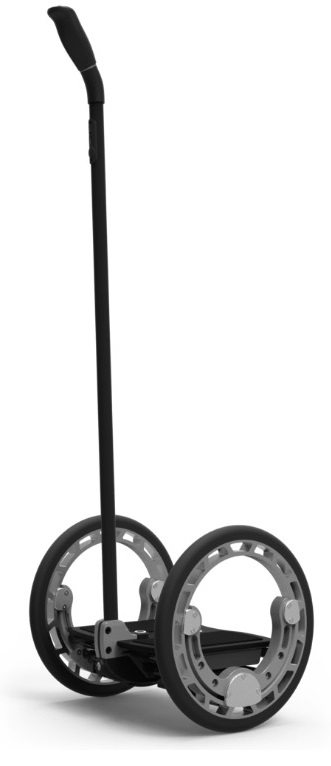
\includegraphics{fig_01}
\end{minipage}
\end{resultat}


\begin{resultat}\textbf{\textsf{\small -- Réponse à une rampe d'un système du premier ordre}}~\\

\noindent \begin{minipage}[c]{.65\linewidth}
On appelle réponse à une rampe, l'expression de la sortie $s$ lorsque on soumet le système à une fonction linéaire de pente $k$: 
$$
S(p)=E(p)H(p) = \dfrac{k}{p^2} \dfrac{K}{1+\tau p}.
$$ 


Analytiquement, on montre que $s(t)=Kk \left(t-\tau+\tau e^{-\frac{t}{\tau}}\right)u(t)$. 

Les caractéristiques de la courbe sont les suivantes : 
\begin{itemize}
\item pente de l'asymptote $K k$;
%\item pente à l'origine \textbf{non nulle};
\item intersection de l'asymptote avec l'axe des abscisses : $t=\tau$;
\item $\varepsilon_{v}=kK\tau$.
%\item Plus $\tau$ est grand, plus le système est lent.
\end{itemize}


\end{minipage} \hfill
\begin{minipage}[c]{.32\linewidth}
\centering
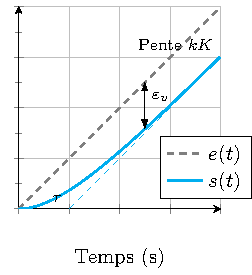
\includegraphics{rampe}
\end{minipage}
\end{resultat}



\section{Systèmes d'ordre 2}

\begin{defi}

Les systèmes du second ordre sont régis par une équation différentielle de la
forme suivante :
$$
\dfrac{1}{\omega_0^2} \dfrac{\dd^2 s(t)}{\dd t^2}+\dfrac{2\xi}{\omega_0} \dfrac{\dd s(t)}{\dd t}+s(t) = Ke(t).
$$

Dans le domaine de Laplace, la fonction de transfert de ce système est donc
donnée par :

\begin{minipage}[c]{.6\linewidth}
$$
H(p)=\dfrac{S(p)}{E(p)} = \dfrac{K}{1+ \dfrac{2\xi}{\omega_0}p+\dfrac{p^2}{\omega_0^2}}.
$$
\end{minipage}\hfill
\begin{minipage}[c]{.35\linewidth}
%Schéma-bloc d'un système du second ordre :

\begin{center}
\begin{tikzpicture}
\sbEntree{E}
\sbBloc[5]{B1}{$\dfrac{K}{1+ \dfrac{2\xi}{\omega_0}p+\dfrac{p^2}{\omega_0^2}}$}{E}
\sbSortie[5]{S}{B1}
\sbRelier[$E(p)$]{E}{B1}
\sbRelier[$S(p)$]{B1}{S}
\end{tikzpicture}
\end{center}
\end{minipage}


On note :
\begin{itemize}
\item $K$ est appelé le gain statique du système (rapport des unités de $S$ et de $E$);
\item $\xi$ (lire \textit{xi}) est appelé coefficient d'amortissement (sans unité);
\item $\omega_0$ pulsation propre du système ($\text{rad/s}$ ou $s^{-1}$).
\end{itemize}


Suivant la valeur du coefficient d'amortissement, l'allure de la réponse temporelle est différente.
\end{defi}

\begin{resultat} ~\\

\vspace*{-1.3cm}

\noindent\begin{center}
\begin{tabular}{p{.4\linewidth}p{.58\linewidth}}
\begin{center}
\textbf{$\xi \geq 1$ : système non oscillant et amorti}

\textbf{(apériodique)}

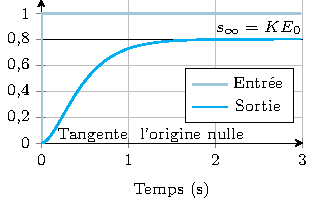
\includegraphics{Ordre2_amorti}
\end{center} 
& 
\begin{center}
\textbf{$\xi <1$ : système oscillant et amorti }

\textbf{(pseudo périodique)}

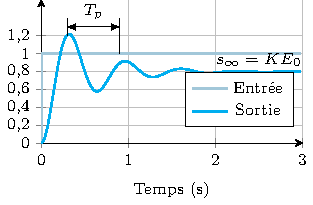
\includegraphics{Ordre2_pseudo}
\end{center} 
\\
\vspace*{-1cm}
\begin{itemize} 
\item La fonction de transfert a deux pôles réels.
\item La tangente à l'origine est nulle.
\end{itemize}
& 
\vspace*{-.8cm}
\begin{itemize} 
\item La fonction de transfert a deux pôles complexes.
\item La tangente à l'origine est nulle.
\item La pseudo-période est de la forme $T_p=\dfrac{2\pi }{\omega_0 \sqrt{1-\xi^2}}$.
\item La valeur du premier dépassement vaut :  $D_1=KE_0e^{\dfrac{-\pi \xi }{\sqrt{1-\xi^2}}}$.
\end{itemize}
\end{tabular}
\end{center}
\end{resultat}

\begin{resultat} ~\\
\vspace{-.2cm}
\begin{itemize}
\item Pour $\xi=0$ le système n'est pas amorti (oscillateur harmonique) la réponse à un échelon est une sinusoïde d'amplitude $KE_0$ ($2KE_0$ crête à crête).  
\item Pour $\xi\simeq 0,69$  on obtient le système du second ordre le plus rapide \textbf{avec dépassement}. 
Le temps de réponse à 5\% est donné par $t_{r 5\%} \cdot \omega_0 \simeq 3$.
\item Pour $\xi =1$ on obtient le système du second ordre le plus rapide \textbf{sans dépassement}.

\end{itemize}
\end{resultat}

